Available resources were always one of the biggest goods Project
Managers had to work with, to keep customers happy. Especially with the growing agile approach
popularity, where development iterations become smaller, it is of high
importance to use all resources the most efficient way. Efficiency in this case,
does not always mean, to put the most fitting developer on a task, but also
consider where the other resources are allocated at the time. Putting a
developer on a task that is not fitting him perfectly might still be a good idea
if another developer would not be able to do anything otherwise.

\section{Methodology of Resource Allocation}
There are various methods which aim at the best possible resource allocation and
they all first require the user, possibly the project manager, to break down
jobs in tasks and classify the tasks and the resources in a specific way. The
better the breakdown and the classification is, the better the project manager
can allocate his resources.

For this project we will use the method described in the lectures of Dr. Ali
Mousavi (see \cite{ResAlloc}). 

This method focuses on classifying tasks and
identifying the best possible human resource to fulfill the task. First the
human resources get their Indicators of Capability:

\begin{itemize}
\item The Enablers (E) � cognitive capabilities, skills and roles
\item The Preferences (P) � personal traits
\item Past Attainments (A) � past experience in similar roles 
\end{itemize}

It takes an experienced project manager and good self-assessment of the
developer to put together a representative and well-founded list of enabler
properties.

In the following, we will calculate the impact and utilization of a specific
human resource on a specific job as an example. Since we are a small company we
take the job implementation as one big job which we separate into tasks (see
figure \ref{fig:table1}). After writing down the most important skills needed 
for the single tasks, we can
put them all together in a separate table, considering the highest $X$ (see
figure \ref{fig:table2}).

\begin{figure}
\centering
\captionsetup{justification=centering}
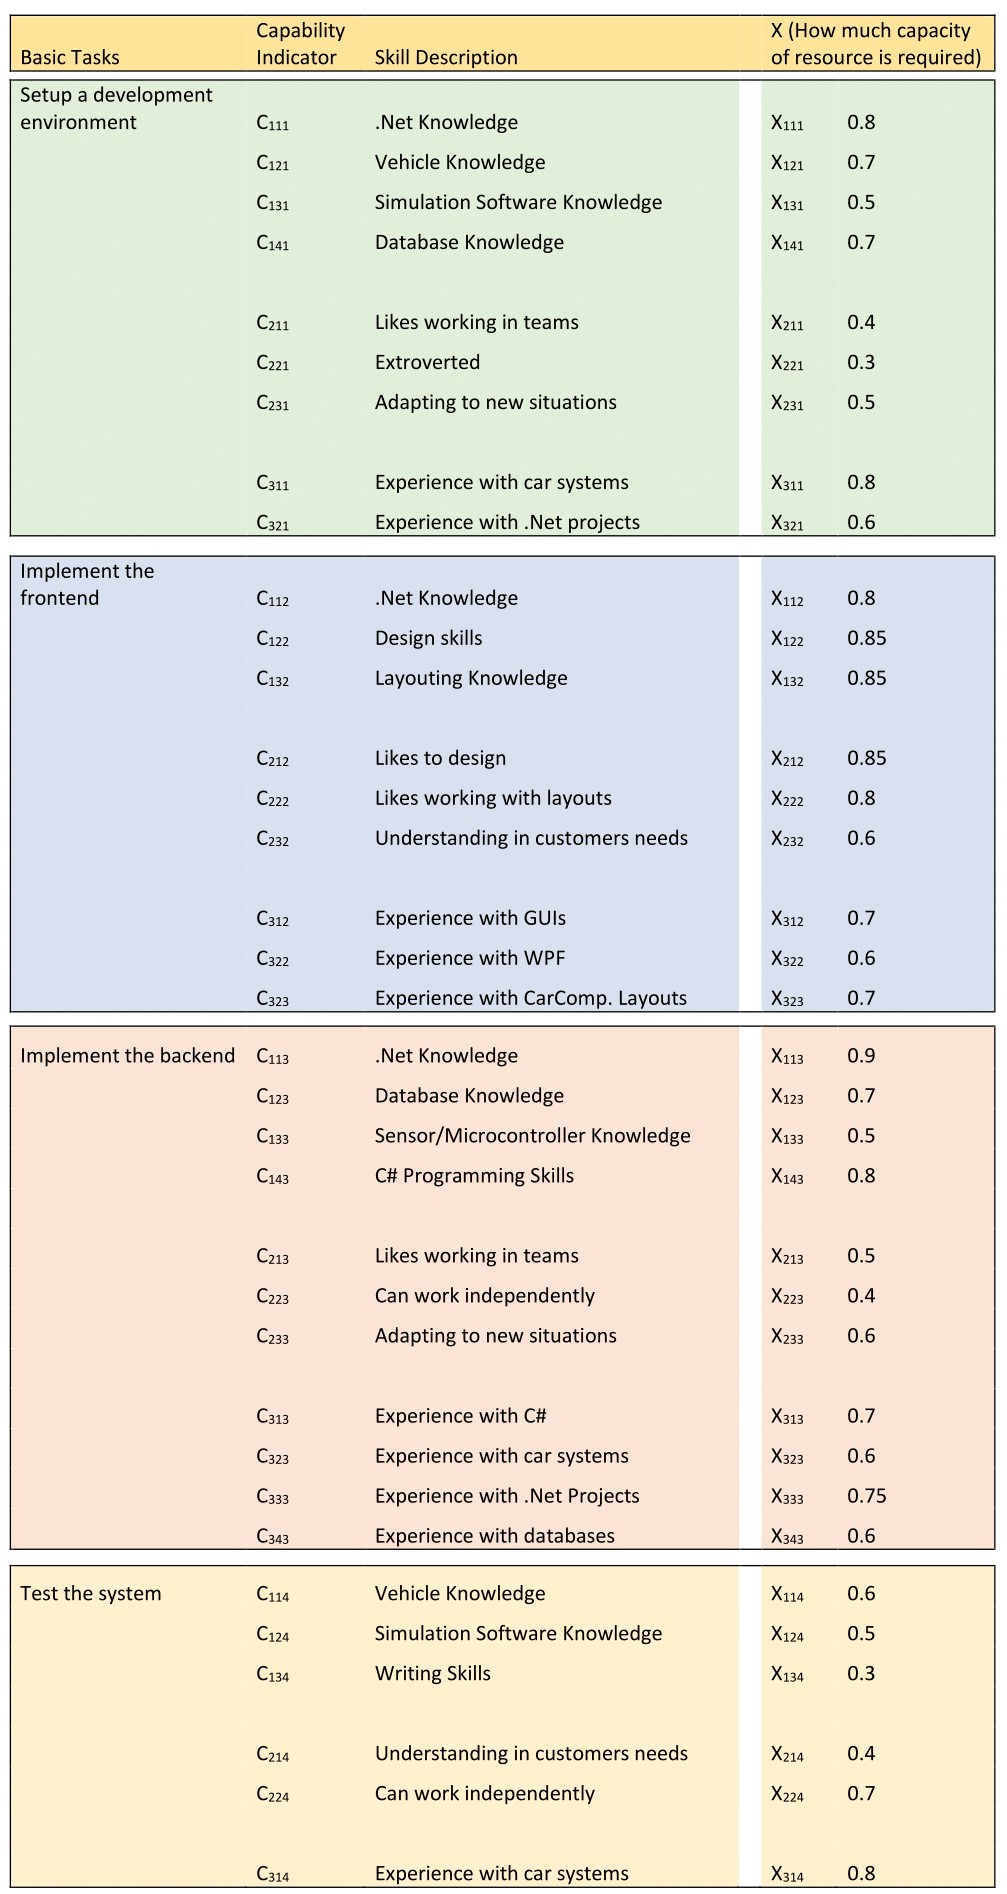
\includegraphics[width=0.75\textwidth]{res/resAlloc/Table1.jpg}
\caption{Task-Resource Matching}
\label{fig:table1}
\end{figure}

\begin{figure}
\centering
\captionsetup{justification=centering}
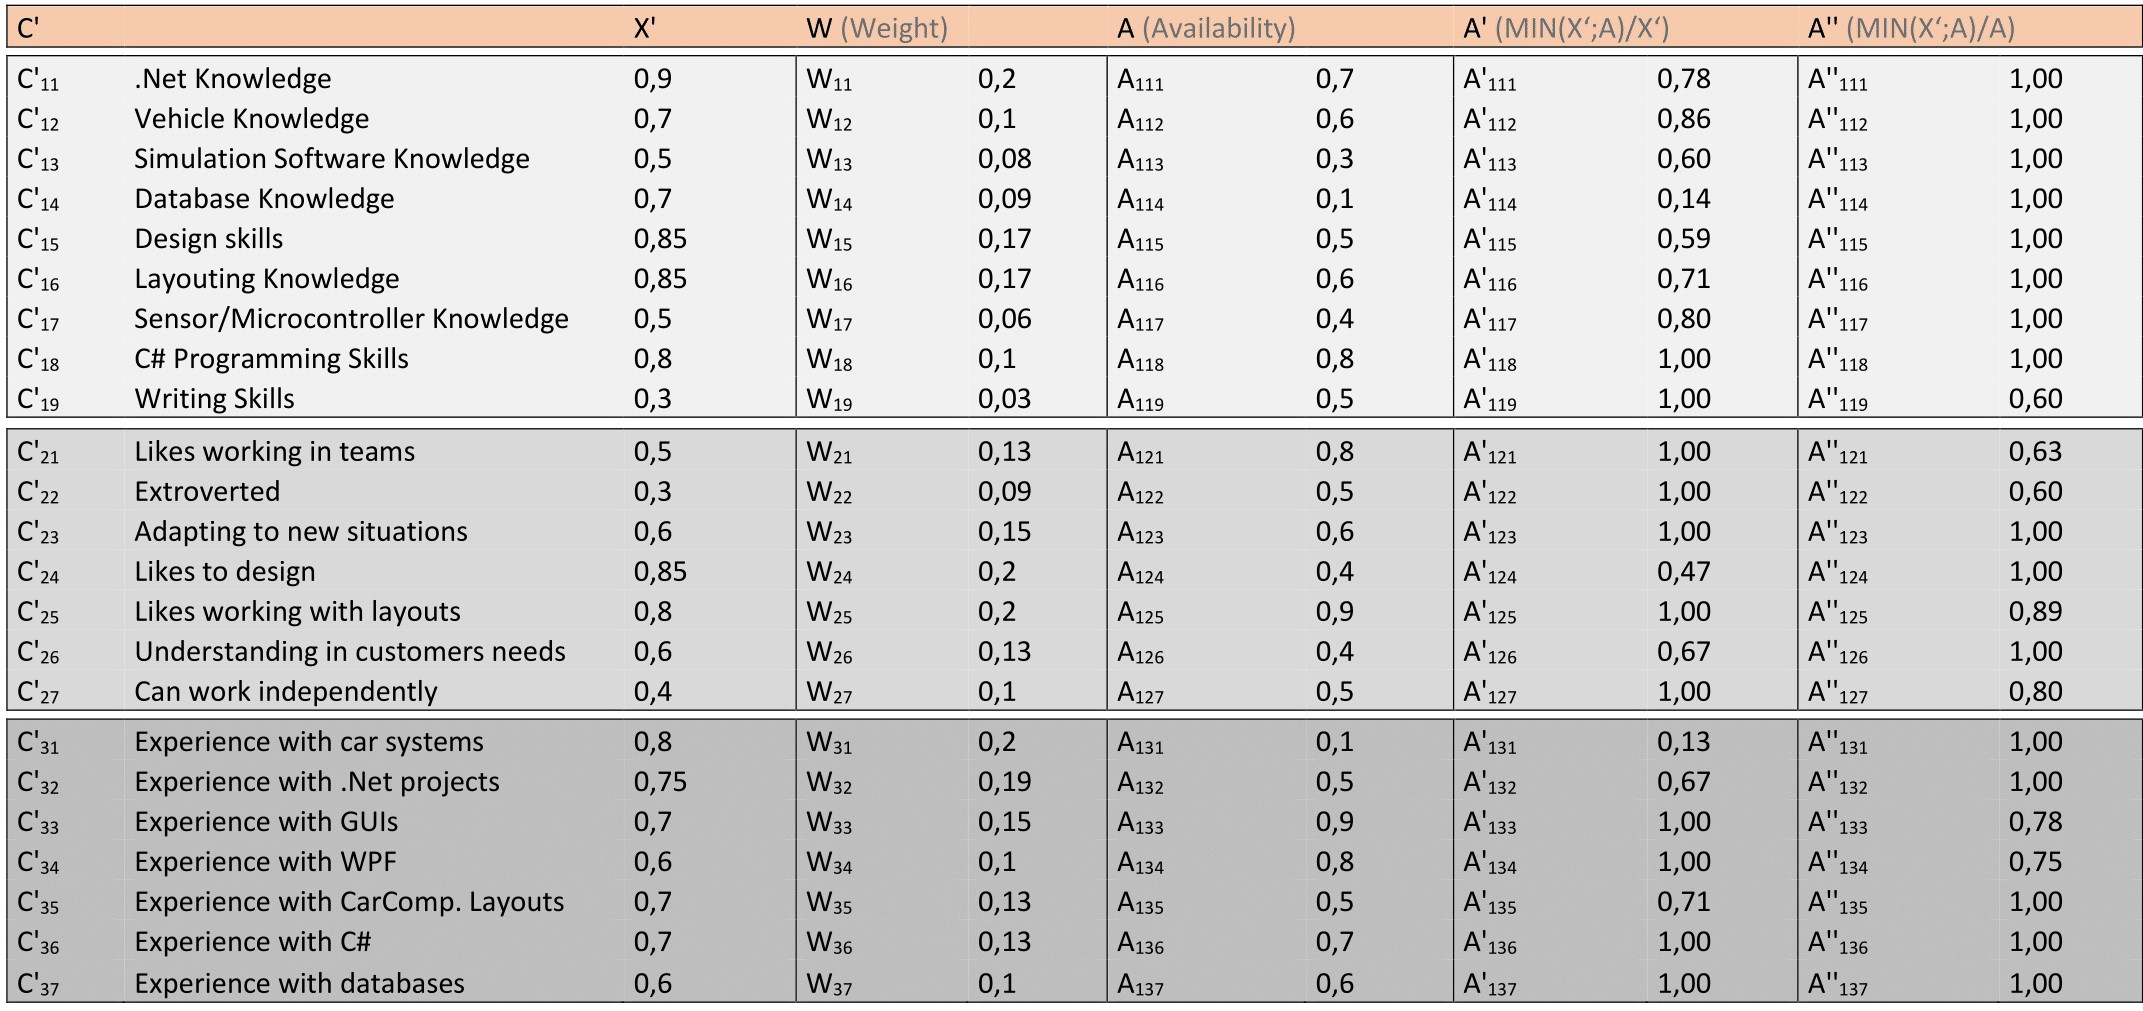
\includegraphics[width=\textwidth]{res/resAlloc/Table2.jpg}
\caption{Individual Availability}
\label{fig:table2}
\end{figure}

Considering the weight of a skill $W$ and the availability of the human resource
$A$ we can calculate the values $A'$ and $A''$. With those values we can calculate 
the Impact and Utilization of a Human
Resource for a job:

\begin{table}[h]
\centering
\captionsetup{justification=centering}
\begin{tabular}{ll}
\textbf{Impact:} & 0.68 \\
\textbf{Utilisation:} & 0.81
\end{tabular}
\caption{Impact and Utilization of a Human Resource}
\label{tab:ImpactAndUtilization}
\end{table}

\begin{figure}
\centering
\captionsetup{justification=centering}
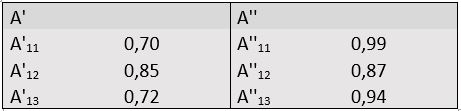
\includegraphics[width=0.75\textwidth]{res/resAlloc/Table3.jpg}
\caption{Normalisation}
\label{fig:table3}
\end{figure}

Those values would have to be compared to the values of other candidates, which
would be too much for this assignment.
